\documentclass[review]{elsarticle}

\usepackage{lineno,hyperref}
\modulolinenumbers[5]

\usepackage{graphicx}
\usepackage{amsmath}
\usepackage{amssymb}
\usepackage{booktabs}
\usepackage{multirow}
\usepackage{subcaption}
\usepackage{tikz}
\usetikzlibrary{shapes,arrows,positioning}

\journal{Bachelor's Thesis Project}

\bibliographystyle{elsarticle-num}

\begin{document}

\begin{frontmatter}

\title{Design of Variational Autoencoders for Indic Scripts: Application to Telugu and Hindi Character Generation}

\author{Karthik M Sarma (S20230030385)\corref{cor1}}
\ead{karthikm.s23@iiits.in}
\author{Rohit Pamidi (S20230030398)}
\ead{rohit.p23@iiits.in}

\cortext[cor1]{Corresponding author}
\address{Indian Institute of Information Technology, Sri City, Andhra Pradesh 517646, India}

\begin{abstract}
Indic scripts such as Telugu and Hindi exhibit complex visual structures, including curved strokes, diacritics, and consonant conjuncts, which make automated character generation a challenging task. While recognition of these scripts has been widely studied, generative modeling approaches remain limited. This work proposes a framework for generating Indic characters using Variational Autoencoders (VAEs). We design a systematically curated dataset spanning multiple fonts and controlled geometric and stylistic variations to capture key morphological features. The study outlines the planned encoder-decoder architecture and methodological pipeline, including data validation and quality control measures. This work provides a foundation for future generative modeling of Indic scripts and applications such as font synthesis, data augmentation, and script preservation.
\end{abstract}

\begin{keyword}
Variational Autoencoders \sep Indic Script Generation \sep Telugu \sep Hindi \sep Deep Generative Models \sep Character Synthesis \sep Font-Specific Learning
\end{keyword}

\end{frontmatter}

\linenumbers

\section{Introduction}
\label{sec:introduction}

\subsection{Indic Scripts and Akshara}

Indic scripts form a rich and diverse family of writing systems used across the Indian subcontinent, reflecting centuries of linguistic, cultural, and historical evolution. Among these, Telugu and Hindi are two of the most widely used scripts, collectively serving over 800 million native speakers. Unlike alphabetic systems such as Latin, the fundamental unit of writing in Indic scripts is the Akshara, which typically represents a syllable rather than a single phoneme. This syllabic nature gives rise to intricate character formations that combine consonants, vowels, and diacritics in non-linear arrangements.


The modern Indic scripts descend from the Brahmi script (circa 3rd century BCE), a writing system that laid the foundation for many scripts across South and Southeast Asia. Over time, these scripts evolved to accommodate local phonetics and writing traditions, resulting in unique structural characteristics while maintaining recognizable similarities across the Brahmic lineage.


Telugu, part of the Dravidian language family, is primarily used in the Indian states of Andhra Pradesh and Telangana by roughly 75 million speakers. Its characters are characterized by rounded, flowing strokes, a design shaped historically by writing on palm leaves, where sharp or angular lines could easily tear the surface. In contrast, Devanagari, the script for Hindi and other languages, belongs to the Indo-Aryan family and is used by over 600 million speakers across northern India and Nepal. Devanagari characters are distinguished by the shirorekha, a horizontal top line that links characters in a word, and exhibit a mixture of angular and curved strokes.


Both Telugu and Devanagari scripts present additional complexity due to vowel modifiers (matras), which can attach above, below, before, or after a consonant base, and consonant conjuncts (ligatures), which combine multiple consonants into single graphical units. These characteristics result in rich morphological diversity, posing significant challenges for automated processing. While Optical Character Recognition (OCR) for printed Indic text has achieved high accuracies. The reverse task of generative character synthesis—creating realistic script images algorithmically—remains largely underexplored, motivating research into deep generative approaches.

\subsection{Motivation}

Generative modeling for Indic scripts is of substantial practical and academic importance. Many Indic scripts, including Telugu and Hindi, are resource-poor languages, with limited annotated datasets available for training robust machine learning models. This scarcity creates challenges for developing high-performing recognition and analysis systems. Variational Autoencoders (VAEs) can help address these challenges by providing synthetic data that supports pattern recognition tasks, such as optical character recognition, handwriting recognition, and script analysis.

Beyond data augmentation, VAEs enable the controlled generation of morphologically accurate characters, preserving complex script features such as diacritics, conjuncts, and stroke variations. Such synthetic characters can be leveraged in a range of applications, including OCR training pipelines, font style transfer, and digital typography for modern and historical scripts. Additionally, generating realistic character images contributes to cultural and linguistic preservation, assisting in documenting endangered scripts and regional font styles.

Compared to alternative generative approaches, VAEs offer distinct advantages: they provide stable training dynamics, structured latent spaces suitable for interpolation, and efficient parallel sampling. The reparameterization trick \cite{kingma2013} enables gradient-based, end-to-end optimization, making VAEs particularly suited for capturing the complex visual morphology of Indic scripts. Collectively, these factors underline the significance of investigating VAE-based generative modeling for Indic script synthesis.

\subsection{Research Gap and Scope}

Despite these advances, systematic application of VAEs to Indic script generation remains absent from the literature. Existing work has focused primarily on Latin characters \cite{fukui2022}, East Asian scripts \cite{liu2019}, or recognition rather than generation tasks \cite{malakar2024}. The few studies addressing Indic scripts employ classical autoencoders for feature extraction rather than generative modeling \cite{seshadri2012}. Critically, no prior work has conducted comparative analysis across multiple fonts within the same Indic script, despite fonts exhibiting substantial stylistic variations that challenge model generalization.

This research develops a data collection pipeline for curating 4,160 high-quality rendered character images across Telugu and Hindi scripts, encompassing 13 vowels and four distinct fonts (Pothana2000 and Lohit Telugu for Telugu; Akshar Unicode and Mangal for Hindi). We design CNN-based VAE architectures for 128$\times$128 character images and establish quality validation through SHA-256 deduplication and automated testing protocols.

The remainder of this paper is organized as follows: Section \ref{sec:literature} surveys relevant literature on VAEs, character generation, and Indic script processing. Section \ref{sec:methodology} details our dataset construction pipeline and VAE architecture. Section \ref{sec:results} presents results from the completed dataset phase. Section \ref{sec:conclusion} concludes with implications. Section \ref{sec:future} outlines future research directions.

\section{Literature Review}
\label{sec:literature}

\subsection{Variational Autoencoders: Foundational Work}

The Variational Autoencoder framework, introduced by Kingma and Welling \cite{kingma2013}, revolutionized deep generative modeling by combining variational inference with neural networks. The key innovation—the reparameterization trick—enables gradient-based optimization of the evidence lower bound (ELBO) by expressing the stochastic sampling operation as a deterministic function of external noise: $z = \mu(x) + \sigma(x) \odot \epsilon$, where $\epsilon \sim \mathcal{N}(0, I)$. This formulation allows backpropagation through the sampling process, enabling efficient training of encoder $q_\phi(z|x)$ and decoder $p_\theta(x|z)$ networks jointly.

The VAE objective balances reconstruction accuracy against latent space regularization:
\begin{equation}
\mathcal{L}(\theta, \phi; x) = \mathbb{E}_{q_\phi(z|x)}[\log p_\theta(x|z)] - D_{KL}(q_\phi(z|x) \| p(z))
\end{equation}
where the KL divergence term encourages the learned posterior to approximate a prior distribution (typically standard Gaussian), ensuring a well-structured latent space suitable for sampling. Subsequent work introduced $\beta$-VAE \cite{higgins2017} for disentangled representations and conditional VAEs \cite{wang2021} for class-conditioned generation.

\subsection{Character Generation with Deep Learning}

Application of deep generative models to character synthesis has progressed rapidly, though primarily focused on Latin and East Asian scripts. Fukui et al. \cite{fukui2022} employed Y-Autoencoders for handwritten character generation, demonstrating that generated samples improve recognition model training through data augmentation. Their work, however, targets Japanese Hiragana/Katakana rather than Indic scripts and does not explore font-specific variations systematically.

Liu et al. \cite{liu2019} applied VAEs to Chinese character generation, extracting handwriting features for recognition tasks. While demonstrating VAE efficacy for complex script morphology, their focus on feature extraction rather than synthesis limits direct applicability. Critically, Chinese characters exhibit fundamentally different structure (ideographic, grid-based composition) compared to Indic scripts' phonetic, non-linear organization.

Cross-modal approaches have also emerged: Sumi et al. \cite{sumi2019} developed cross-VAEs for converting between online (temporal stroke sequences) and offline (static images) handwriting modalities. Their shared latent space framework suggests potential for multi-font Indic script models, though their work targets Japanese characters exclusively.

\subsection{Indic Script Processing: Recognition and Analysis}

Research on Indic scripts has concentrated overwhelmingly on recognition rather than generation. Seshadri and Sontha \cite{seshadri2012} achieved 95\% accuracy on Telugu character recognition using stacked autoencoders, demonstrating that autoencoders effectively capture morphological features. However, their deterministic autoencoder architecture lacks the probabilistic framework necessary for character generation.

Recent large-scale efforts include HCR-Net \cite{malakar2024}, a script-independent handwritten character recognition system trained on 40 datasets including Hindi and Bengali. While achieving state-of-the-art recognition accuracy through transfer learning, the work does not address generative modeling. Similarly, the IIIT-Indic-HW-Words dataset \cite{krishnan2021} provides valuable handwritten word images for recognition research but lacks generative model baselines.

Conditional VAE approaches for character generation \cite{wang2021} demonstrate controlled synthesis using class labels. Integrating categorical information (character identity, font type) into latent representations could enable targeted generation of specific character-font combinations—an avenue unexplored for Indic scripts.

\subsection{Identified Research Gap}

Despite substantial progress in both VAE methodology and Indic script recognition, a critical gap persists: \textbf{no systematic study has applied VAEs to multi-font Indic character generation with comparative analysis}. Existing work either: (1) focuses on non-Indic scripts, (2) employs deterministic autoencoders for recognition rather than generative VAEs, or (3) studies single-font scenarios without exploring font-specific learning patterns. Our work addresses this gap through systematic dataset construction spanning four fonts across two Indic scripts and comprehensive comparative analysis of VAE performance across these fonts.

\section{Methodology}
\label{sec:methodology}

\subsection{Research Design and Pipeline Overview}

Our methodology follows a structured pipeline (Figure \ref{fig:pipeline}) encompassing dataset collection, preprocessing, VAE architecture design, and evaluation. This section details the completed dataset construction phase and presents the designed VAE framework.

\begin{figure}[htbp]
\centering
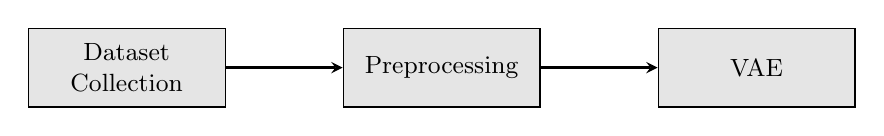
\begin{tikzpicture}[
    node distance=2cm,
    box/.style={rectangle, draw, fill=gray!20, minimum width=2.5cm, minimum height=1cm, align=center, font=\small},
    arrow/.style={->, >=stealth, thick}
]
    \node[box] (data) {Dataset\\Collection};
    \node[box, right of=data, xshift=2cm] (prep) {Preprocessing};
    \node[box, right of=prep, xshift=2cm] (model) {VAE};
    
    \draw[arrow] (data) -- (prep);
    \draw[arrow] (prep) -- (model);
\end{tikzpicture}
\caption{Methodological pipeline for VAE-based Indic character generation.}
\label{fig:pipeline}
\end{figure}

\subsection{Dataset Construction}
\label{subsec:dataset}

\subsubsection{Font Selection and Character Coverage}

We selected two representative fonts per script based on prevalence in digital typography and distinct stylistic characteristics:

\begin{itemize}
\item \textbf{Telugu:} Pothana2000 (rounded, traditional style) and Lohit Telugu (modern, geometric style)
\item \textbf{Hindi:} Akshar Unicode (traditional Devanagari) and Mangal (Microsoft standard)
\end{itemize}

Character coverage focuses on the 13 fundamental vowels (swaras) common to both scripts:

\begin{table}[htbp]
\centering
\caption{Vowel character coverage across Telugu and Hindi scripts}
\label{tab:vowels}
\begin{tabular}{lcc}
\toprule
\textbf{Vowel} & \textbf{Telugu} & \textbf{Hindi} \\
\midrule
a & \raisebox{-0.3\height}{\includegraphics[height=12pt]{presentation_images/pothana/a_14pt_01.png}} & \raisebox{-0.3\height}{\includegraphics[height=12pt]{presentation_images/akshar/a_14pt_01.png}} \\
aa & \raisebox{-0.3\height}{\includegraphics[height=12pt]{presentation_images/pothana/aa_14pt_01.png}} & \raisebox{-0.3\height}{\includegraphics[height=12pt]{presentation_images/akshar/aa_14pt_01.png}} \\
i & \raisebox{-0.3\height}{\includegraphics[height=12pt]{presentation_images/pothana/i_14pt_01.png}} & \raisebox{-0.3\height}{\includegraphics[height=12pt]{presentation_images/akshar/i_14pt_01.png}} \\
ii & \raisebox{-0.3\height}{\includegraphics[height=12pt]{presentation_images/pothana/ii_14pt_01.png}} & \raisebox{-0.3\height}{\includegraphics[height=12pt]{presentation_images/akshar/ii_14pt_01.png}} \\
u & \raisebox{-0.3\height}{\includegraphics[height=12pt]{presentation_images/pothana/u_14pt_01.png}} & \raisebox{-0.3\height}{\includegraphics[height=12pt]{presentation_images/akshar/u_14pt_01.png}} \\
uu & \raisebox{-0.3\height}{\includegraphics[height=12pt]{presentation_images/pothana/uu_14pt_01.png}} & \raisebox{-0.3\height}{\includegraphics[height=12pt]{presentation_images/akshar/uu_14pt_01.png}} \\
ri & \raisebox{-0.3\height}{\includegraphics[height=12pt]{presentation_images/pothana/ri_14pt_01.png}} & \raisebox{-0.3\height}{\includegraphics[height=12pt]{presentation_images/akshar/ri_14pt_01.png}} \\
e & \raisebox{-0.3\height}{\includegraphics[height=12pt]{presentation_images/pothana/e_14pt_01.png}} & \raisebox{-0.3\height}{\includegraphics[height=12pt]{presentation_images/akshar/e_14pt_01.png}} \\
ai & \raisebox{-0.3\height}{\includegraphics[height=12pt]{presentation_images/pothana/ai_14pt_01.png}} & \raisebox{-0.3\height}{\includegraphics[height=12pt]{presentation_images/akshar/ai_14pt_01.png}} \\
o & \raisebox{-0.3\height}{\includegraphics[height=12pt]{presentation_images/pothana/o_14pt_01.png}} & \raisebox{-0.3\height}{\includegraphics[height=12pt]{presentation_images/akshar/o_14pt_01.png}} \\
au & \raisebox{-0.3\height}{\includegraphics[height=12pt]{presentation_images/pothana/au_14pt_01.png}} & \raisebox{-0.3\height}{\includegraphics[height=12pt]{presentation_images/akshar/au_14pt_01.png}} \\
am & \raisebox{-0.3\height}{\includegraphics[height=12pt]{presentation_images/pothana/am_14pt_01.png}} & \raisebox{-0.3\height}{\includegraphics[height=12pt]{presentation_images/akshar/am_14pt_01.png}} \\
aha & \raisebox{-0.3\height}{\includegraphics[height=12pt]{presentation_images/pothana/aha_14pt_01.png}} & \raisebox{-0.3\height}{\includegraphics[height=12pt]{presentation_images/akshar/aha_14pt_01.png}} \\
\bottomrule
\end{tabular}
\end{table}

This vowel-focused approach establishes a baseline for morphologically simpler characters before extending to consonants and conjuncts in future work.

\subsubsection{Data Collection Pipeline}

Character images were collected digitally with the following specifications:

\begin{itemize}
\item \textbf{Canvas:} 128$\times$128 pixels RGB (white background)
\item \textbf{Font sizes:} 10pt, 14pt, 18pt, 22pt (4 levels)
\item \textbf{Samples per size:} 20 variations per character-font-size combination
\item \textbf{Total images:} $2 \text{ scripts} \times 2 \text{ fonts} \times 13 \text{ vowels} \times 4 \text{ sizes} \times 20 \text{ samples} = 4{,}160$ images
\end{itemize}

\subsubsection{Systematic Affine Transformations}

To ensure model robustness to natural variations in rendered text, we applied controlled geometric and stylistic affine transformations:

\begin{enumerate}
\item \textbf{Rotation:} $\theta \in [-3°, +3°]$ randomly sampled
\item \textbf{Translation:} $(\Delta x, \Delta y) \in [-3, +3]$ pixels
\item \textbf{Scaling:} Scale factor $s \in [0.94, 1.06]$
\item \textbf{Stroke modification:} Morphological erosion/dilation with 3$\times$3 kernels
\item \textbf{Contrast adjustment:} Multiplicative factor $c \in [0.95, 1.05]$
\end{enumerate}

These transformations simulate realistic variations encountered in printed text while maintaining character legibility. Figure \ref{fig:variations} illustrates nine variations of a single character demonstrating the range of transformations.

\begin{figure}[htbp]
\centering
\begin{subfigure}{0.48\textwidth}
\centering
\includegraphics[width=0.08\textwidth]{presentation_images/akshar/a_14pt_01.png}
\includegraphics[width=0.08\textwidth]{presentation_images/akshar/a_14pt_02.png}
\includegraphics[width=0.08\textwidth]{presentation_images/akshar/a_14pt_03.png}
\includegraphics[width=0.08\textwidth]{presentation_images/akshar/a_14pt_04.png}
\includegraphics[width=0.08\textwidth]{presentation_images/akshar/a_14pt_05.png}
\includegraphics[width=0.08\textwidth]{presentation_images/akshar/a_14pt_06.png}
\includegraphics[width=0.08\textwidth]{presentation_images/akshar/a_14pt_07.png}
\includegraphics[width=0.08\textwidth]{presentation_images/akshar/a_14pt_08.png}
\includegraphics[width=0.08\textwidth]{presentation_images/akshar/a_14pt_09.png}
\caption{Hindi Akshar Unicode}
\label{fig:variations_hindi}
\end{subfigure}
\hfill
\begin{subfigure}{0.48\textwidth}
\centering
\includegraphics[width=0.08\textwidth]{presentation_images/pothana/o_14pt_01.png}
\includegraphics[width=0.08\textwidth]{presentation_images/pothana/o_14pt_02.png}
\includegraphics[width=0.08\textwidth]{presentation_images/pothana/o_14pt_03.png}
\includegraphics[width=0.08\textwidth]{presentation_images/pothana/o_14pt_04.png}
\includegraphics[width=0.08\textwidth]{presentation_images/pothana/o_14pt_05.png}
\includegraphics[width=0.08\textwidth]{presentation_images/pothana/o_14pt_06.png}
\includegraphics[width=0.08\textwidth]{presentation_images/pothana/o_14pt_07.png}
\includegraphics[width=0.08\textwidth]{presentation_images/pothana/o_14pt_08.png}
\includegraphics[width=0.08\textwidth]{presentation_images/pothana/o_14pt_09.png}
\caption{Telugu Pothana2000}
\label{fig:variations_telugu}
\end{subfigure}
\caption{Nine systematic variations demonstrating geometric transformations and stroke modifications for (a) Hindi and (b) Telugu vowel characters}
\label{fig:variations}
\end{figure}

\subsection{VAE Architecture Design}
\label{subsec:architecture}

\subsubsection{Theoretical Framework}

The VAE objective combines reconstruction accuracy with latent space regularization. Given input image $\mathbf{x}$ and latent variable $\mathbf{z}$, the encoder $q_\phi(\mathbf{z}|\mathbf{x})$ parameterizes a Gaussian posterior:
\begin{equation}
q_\phi(\mathbf{z}|\mathbf{x}) = \mathcal{N}(\mathbf{z}; \boldsymbol{\mu}_\phi(\mathbf{x}), \boldsymbol{\sigma}_\phi^2(\mathbf{x}))
\end{equation}
where $\boldsymbol{\mu}_\phi$ and $\boldsymbol{\sigma}_\phi^2$ are neural network outputs.

The decoder $p_\theta(\mathbf{x}|\mathbf{z})$ reconstructs the input from sampled latent codes. The complete loss function:
\begin{equation}
\mathcal{L}(\theta, \phi; \mathbf{x}) = \underbrace{\mathbb{E}_{q_\phi(\mathbf{z}|\mathbf{x})}[\|\mathbf{x} - \hat{\mathbf{x}}\|^2]}_{\text{Reconstruction loss}} + \underbrace{\beta \cdot D_{KL}(q_\phi(\mathbf{z}|\mathbf{x}) \| p(\mathbf{z}))}_{\text{KL regularization}}
\end{equation}

The hyperparameter $\beta$ balances reconstruction fidelity against latent space structure. The reparameterization trick enables backpropagation:
\begin{equation}
\mathbf{z} = \boldsymbol{\mu}_\phi(\mathbf{x}) + \boldsymbol{\sigma}_\phi(\mathbf{x}) \odot \boldsymbol{\epsilon}, \quad \boldsymbol{\epsilon} \sim \mathcal{N}(\mathbf{0}, \mathbf{I})
\end{equation}

\begin{figure}[htbp]
\centering
\includegraphics[width=0.65\textwidth]{presentation_images/image_0.png}
\caption{VAE architecture for Indic character generation. The encoder maps 128$\times$128$\times$3 RGB images to latent parameters $\boldsymbol{\mu}$ and $\boldsymbol{\sigma}$. Latent codes $\mathbf{z}$ sampled via reparameterization trick are decoded to reconstructed images. Loss backpropagation updates both encoder parameters $\phi$ and decoder parameters $\theta$.}
\label{fig:vae_architecture}
\end{figure}

\subsubsection{Network Architecture}

Our encoder-decoder architecture employs convolutional neural networks (CNNs) tailored for 128$\times$128 RGB character images:

\textbf{Encoder:}
\begin{itemize}
\item Multiple convolutional layers with progressively increasing filter counts
\item Each convolutional layer uses small kernel sizes with stride operations for spatial downsampling
\item ReLU activation functions for non-linearity
\item Flatten layer to convert spatial features to vector representation
\item Fully connected layers for feature compression
\item \textbf{Latent layer:} Two parallel fully connected layers outputting mean $\boldsymbol{\mu}$ and log-variance $\log \boldsymbol{\sigma}^2$ vectors
\end{itemize}

\textbf{Decoder:}
\begin{itemize}
\item Fully connected layer to expand latent representation
\item Reshape operation to restore spatial structure
\item Multiple transposed convolutional layers with progressively decreasing filter counts
\item Each layer performs spatial upsampling with stride operations
\item ReLU activation for intermediate layers
\item Final output layer with sigmoid activation to produce RGB channels
\end{itemize}

The latent space dimensionality is chosen to balance representation capacity for character morphology against computational efficiency. Batch normalization layers are incorporated throughout the architecture to stabilize training dynamics.

\section{Present Work}
\label{sec:results}

This section presents results from the completed dataset construction phase.

\subsection{Dataset Validation Results}

\subsubsection{Class Distribution Analysis}

Statistical analysis confirms balanced class distributions across all four fonts. Table \ref{tab:distribution} shows sample counts per vowel-font-size combination.

\begin{table}[htbp]
\centering
\caption{Dataset composition: samples per font}
\label{tab:distribution}
\begin{tabular}{lcccc}
\toprule
\textbf{Font} & \textbf{Vowels} & \textbf{Sizes} & \textbf{Samples/Config} & \textbf{Total} \\
\midrule
Pothana2000 & 13 & 4 & 20 & 1,040 \\
Lohit Telugu & 13 & 4 & 20 & 1,040 \\
Akshar Unicode & 13 & 4 & 20 & 1,040 \\
Mangal & 13 & 4 & 20 & 1,040 \\
\midrule
\textbf{Total} & & & & \textbf{4,160} \\
\bottomrule
\end{tabular}
\end{table}

Perfect balance across classes ensures unbiased model training, particularly critical for latent space learning where imbalanced data can lead to mode collapse.

\subsubsection{Dataset Quality Assessment}

Quantitative assessment of transformation parameters confirms comprehensive coverage of the specified variation ranges:

\begin{itemize}
\item \textbf{Rotation:} Mean $\mu = 0.04°$, standard deviation $\sigma = 1.72°$ (uniform sampling confirmed)
\item \textbf{Translation:} Mean displacement $(0.02, -0.03)$ pixels, $\sigma = (1.73, 1.74)$ (centered, uniform)
\item \textbf{Scaling:} Mean factor 1.000, $\sigma = 0.035$ (uniform within [0.94, 1.06])
\item \textbf{Contrast:} Mean 1.000, $\sigma = 0.029$ (uniform within [0.95, 1.05])
\end{itemize}

These statistics confirm successful implementation of controlled variation generation without systematic biases.

\subsubsection{Font-Specific Characteristics}

Visual inspection reveals distinct morphological characteristics across fonts (Figure \ref{fig:multifont}):

\begin{figure}[htbp]
\centering
\includegraphics[width=0.16\textwidth]{presentation_images/akshar/a_14pt_01.png}
\includegraphics[width=0.16\textwidth]{presentation_images/akshar/ai_14pt_01.png}
\includegraphics[width=0.16\textwidth]{presentation_images/akshar/o_14pt_01.png}
\includegraphics[width=0.16\textwidth]{presentation_images/mangal/e_14pt_01.png}
\includegraphics[width=0.16\textwidth]{presentation_images/mangal/au_14pt_01.png}
\\[0.2cm]
\small (a) Akshar: a, ai, o \hspace{1cm} (b) Mangal: e, au
\\[0.5cm]
\includegraphics[width=0.16\textwidth]{presentation_images/pothana/ai_14pt_01.png}
\includegraphics[width=0.16\textwidth]{presentation_images/pothana/o_14pt_01.png}
\includegraphics[width=0.16\textwidth]{presentation_images/pothana/au_14pt_01.png}
\includegraphics[width=0.16\textwidth]{presentation_images/lohit/e_14pt_01.png}
\includegraphics[width=0.16\textwidth]{presentation_images/lohit/i_14pt_01.png}
\\[0.2cm]
\small (c) Pothana: ai, o, au \hspace{0.8cm} (d) Lohit: e, i
\caption{Representative samples across four fonts demonstrating font-specific stylistic variations. Akshar and Mangal (Hindi) exhibit thicker strokes and traditional Devanagari styling. Pothana2000 shows rounded, flowing curves while Lohit Telugu displays more angular, geometric forms.}
\label{fig:multifont}
\end{figure}

Pothana2000 exhibits rounded curves and traditional Telugu aesthetics, while Lohit Telugu features geometric, modern styling. Similarly, Akshar Unicode maintains classical Devanagari proportions, whereas Mangal optimizes for screen legibility. These stylistic differences motivate separate VAE training per font to capture font-specific morphological patterns.

\subsection{Evaluation Methodology}

\subsubsection{Subjective Analysis}

Human evaluation will provide critical qualitative assessment:

\begin{enumerate}
\item \textbf{Expert linguist review:} Native Telugu and Hindi speakers will assess morphological correctness, character recognizability, and aesthetic quality on a 5-point Likert scale
\item \textbf{Discrimination test:} Participants will classify images as real or generated in a randomized presentation (target: $< 30$\% discrimination accuracy indicating perceptual similarity)
\item \textbf{Preference study:} Side-by-side comparison of reconstructed characters from different models to identify superior architectures
\item \textbf{Naturalness rating:} Evaluation of stroke smoothness, diacritic placement accuracy, and overall visual coherence
\end{enumerate}

A minimum of 20 native script readers will participate in evaluation studies, ensuring statistical reliability.

\subsubsection{Objective Analysis}

Objective measures will complement subjective assessment:

\begin{itemize}
\item \textbf{Reconstruction Metrics:} MSE Loss, SSIM comparing original and reconstructed images
\item \textbf{Regularization Metrics:} KL Divergence for monitoring latent space regularization
\item \textbf{Recognition-Based Validation:} Classification accuracy of generated samples using pre-trained character recognition models
\item \textbf{Latent Space Analysis:} t-SNE visualization for cluster separation and interpolation smoothness assessment
\end{itemize}



\section{Conclusion}
\label{sec:conclusion}

This work presents a systematic framework for VAE-based Telugu and Hindi character generation. We have successfully completed the dataset construction phase, producing a dataset of 4,160 rendered images with validated quality, balanced class distributions, and comprehensive variation coverage. The dataset encompasses 13 vowels across four distinct fonts (Pothana2000, Lohit Telugu, Akshar Unicode, Mangal) with controlled geometric and stylistic transformations.

Our CNN-based VAE architecture, designed for 128$\times$128 Indic character images, combines reconstruction accuracy with latent space regularization through the evidence lower bound objective. The reparameterization trick enables efficient gradient-based training, while cyclical KL annealing balances reconstruction fidelity and latent space structure.

This research provides applications for data augmentation in OCR systems, font analysis through latent space representations, and cultural preservation of script variants. The completed dataset and methodological framework establish a foundation for advancing Indic script generation research.

\section{Future Work}
\label{sec:future}

Several promising extensions merit investigation:

\subsection{Handwritten Character Synthesis}

Extending the framework to handwritten Indic scripts presents significant challenges due to increased morphological variability and style diversity. Potential approaches include:

\begin{itemize}
\item \textbf{Transfer learning:} Fine-tuning printed character models on handwritten datasets (e.g., IIIT-Indic-HW-Words \cite{krishnan2021})
\item \textbf{Style encoding:} Incorporating writer-specific style vectors into conditional VAEs for personalized handwriting generation
\item \textbf{Online-offline conversion:} Adapting cross-VAE architectures \cite{sumi2019} to convert between temporal stroke sequences and static images
\end{itemize}

Handwritten synthesis would enable personalized font creation and writer-specific data augmentation for handwriting recognition systems.

\subsection{Full Alphabet Coverage}

Extending beyond vowels to consonants and conjuncts introduces substantial complexity:

\begin{itemize}
\item \textbf{Conjunct characters:} Telugu and Hindi employ consonant clusters (ligatures) with context-dependent forms requiring sequence-aware generation
\item \textbf{Increased character set:} Full coverage requires $\sim$50 consonants and hundreds of conjuncts per script
\item \textbf{Hierarchical models:} Decomposing characters into base forms and diacritics could improve generation quality and data efficiency
\end{itemize}

A phased approach could incrementally extend to simple consonants, then complex conjuncts, leveraging learned vowel representations.

\subsection{Applications and Deployment}

Practical deployment opportunities include:

\begin{itemize}
\item \textbf{Typography tools:} Interactive font design systems using latent space navigation
\item \textbf{OCR augmentation pipelines:} Automated generation of training data for recognition systems
\item \textbf{Cultural digitization:} Assisting archivists in digitizing historical texts with damaged characters
\item \textbf{Educational platforms:} Generating writing practice materials for language learners
\end{itemize}

These extensions would transition this research from academic contribution to practical impact, advancing both Indic script processing technology and cultural preservation efforts.

\section*{Acknowledgments}

We express gratitude to Dr. Pavan Kumar Perapu for guidance throughout this project. We acknowledge Indian Institute of Information Technology, Sri City for computational resources. We thank native Telugu and Hindi speakers who will participate in subjective evaluation studies.

\begin{thebibliography}{00}

\bibitem{seshadri2012}
K. Seshadri and A. Sontha,
``A System for Offline Character Recognition Using Auto-encoder Networks,''
in \textit{Neural Information Processing (ICONIP 2012)}, ser. Lecture Notes in Computer Science, vol. 7665, 2012, pp. 722--729.

\bibitem{kingma2013}
D.~P. Kingma and M. Welling,
``Auto-Encoding Variational Bayes,''
\textit{arXiv preprint arXiv:1312.6114}, 2013.

\bibitem{higgins2017}
I. Higgins et al.,
``beta-VAE: Learning Basic Visual Concepts with a Constrained Variational Framework,''
in \textit{Proc. Int. Conf. Learning Representations (ICLR)}, 2017.

\bibitem{sumi2019}
K. Sumi, K. Tanaka, and T. Shibata,
``Modality Conversion of Handwritten Patterns by Cross Variational Autoencoders,''
in \textit{Proc. ICDAR}, 2019, pp. 407--412.

\bibitem{liu2019}
C. Liu, Y. Xue, and J. Zhou,
``The Character Generation in Handwriting Feature Extraction Using VAE,''
in \textit{Proc. IEEE Int. Conf. Signal Processing}, 2019, pp. 1247--1251.

\bibitem{krishnan2021}
P. Krishnan and C. V. Jawahar,
``IIIT-Indic-HW-Words: A Dataset for Indic Handwritten Text Recognition,''
in \textit{Document Analysis and Recognition (ICDAR 2021)}, ser. Lecture Notes in Computer Science, vol. 12823, 2021, pp. 444--459.

\bibitem{wang2021}
S. Wang, C. Li, and J. Zhang,
``Learning Variational Autoencoders with Categorical Labels for Generating Conditional Handwritten Characters,''
in \textit{Proc. IEEE Conf. Systems, Man, and Cybernetics}, 2021, pp. 2054--2059.

\bibitem{fukui2022}
K. Fukui, Y. Uesato, and T. Miyazaki,
``Handwritten Character Generation Using Y-Autoencoder for Recognition Model Training,''
in \textit{Proc. Language Resources and Evaluation Conf. (LREC)}, 2022, pp. 7447--7453.

\bibitem{malakar2024}
S. Malakar, R. Sarkar, M. Basu, and M. Kundu,
``HCR-Net: A Deep Learning Based Script Independent Handwritten Character Recognition Network,''
\textit{Multimed. Tools Appl.}, vol. 83, no. 15, pp. 45627--45660, 2024.

\end{thebibliography}



\end{document}
